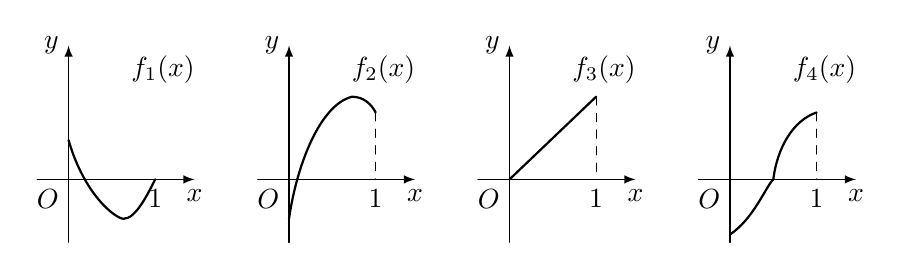
\begin{tikzpicture}[>=latex, scale=1.0, line join=round, line cap=round]
  % Subplot 1: f1(x)
  \begin{scope}[shift={(0, 0)}]
    \draw[->] (-0.4, 0) -- (1.6, 0) node[below] {$x$};
    \draw[->] (0, -0.8) -- (0, 1.7) node[left] {$y$};
    \node[below left] at (0, 0) {$O$};
    \draw[thick] (0, 0.5) .. controls (0.2, -0.2) and (0.6, -0.5) .. (0.7, -0.5)
      .. controls (0.85, -0.5) and (1.0, -0.2) .. (1.1, 0);
    \node[below] at (1.1, 0) {$1$};
    \node[above] at (1.2, 1.1) {$f_1(x)$};
  \end{scope}

  % Subplot 2: f2(x)
  \begin{scope}[shift={(2.8, 0)}]
    \draw[->] (-0.4, 0) -- (1.6, 0) node[below] {$x$};
    \draw[->] (0, -0.8) -- (0, 1.7) node[left] {$y$};
    \node[below left] at (0, 0) {$O$};
    \draw[thick] (0, -0.5) .. controls (0.1, 0.2) and (0.4, 0.95) .. (0.8, 1.05)
      .. controls (0.95, 1.05) and (1.05, 0.95) .. (1.1, 0.85);
    \draw[dashed, thin] (1.1, 0.85) -- (1.1, 0);
    \node[below] at (1.1, 0) {$1$};
    \node[above] at (1.2, 1.1) {$f_2(x)$};
  \end{scope}

  % Subplot 3: f3(x)
  \begin{scope}[shift={(5.6, 0)}]
    \draw[->] (-0.4, 0) -- (1.6, 0) node[below] {$x$};
    \draw[->] (0, -0.8) -- (0, 1.7) node[left] {$y$};
    \node[below left] at (0, 0) {$O$};
    \draw[thick] (0, 0) -- (1.1, 1.05);
    \draw[dashed, thin] (1.1, 1.05) -- (1.1, 0);
    \node[below] at (1.1, 0) {$1$};
    \node[above] at (1.2, 1.1) {$f_3(x)$};
  \end{scope}

  % Subplot 4: f4(x)
  \begin{scope}[shift={(8.4, 0)}]
    \draw[->] (-0.4, 0) -- (1.6, 0) node[below] {$x$};
    \draw[->] (0, -0.8) -- (0, 1.7) node[left] {$y$};
    \node[below left] at (0, 0) {$O$};
    \draw[thick] (0, -0.7) .. controls (0.3, -0.5) and (0.45, -0.1) .. (0.55, 0)
      .. controls (0.6, 0.4) and (0.8, 0.75) .. (1.1, 0.85);
    \draw[dashed, thin] (1.1, 0.85) -- (1.1, 0);
    \node[below] at (1.1, 0) {$1$};
    \node[above] at (1.2, 1.1) {$f_4(x)$};
  \end{scope}
\end{tikzpicture}
